\documentclass[a4paper]{article} 
\usepackage[14pt]{extsizes} % для того чтобы задать нестандартный 14-ый размер шрифта 
\usepackage[utf8]{inputenc} 
\usepackage[russian]{babel} 
\usepackage{amsmath,amsfonts,amssymb,amsthm,mathtools} 
\usepackage[left=20mm, top=15mm, right=15mm, bottom=15mm, nohead, footskip=10mm]{geometry} % настройки полей документа 

\begin{document} % начало документа 
% НАЧАЛО ТИТУЛЬНОГО ЛИСТА 
\begin{center} 
\hfill \break 
\large{Санкт-Петербургский Политехнический университет имени Петра Великого}\\ 
 
 \hfill \break 
\hfill\break 
\hfill \break 
\hfill \break 
\hfill \break 
\begin{center}\large{Отчёт по лабораторной работе №4} \end{center}  
\hfill \break 
\large{Тема: Численное интегрирование} 
\hfill \break 
\hfill \break 
 
\hfill \break 
\hfill \break 
\\ 
\hfill \break 
\hfill \break 
\end{center} 


\normalsize{ 
\begin{tabular}{cccc} 
Студент & : & Алексеева Мария Сергеевна\\\\ 
Группа & : & 5030103/00003 \\\\ 
Преподаватель & : & Козлов Константин Николаевич \\\\ 
\end{tabular} 
}\\ 
\hfill \break 
\hfill \break 
\hfill \break 
\begin{center} Санкт-Петербург 2022 \end{center} 
\thispagestyle{empty} % выключаем отображение номера для этой страницы 
 
% КОНЕЦ ТИТУЛЬНОГО ЛИСТА 
\newpage 
	
\section{Формулировка задачи и её формализация} 
Задача: Вычислить значение интеграла функции $y = x^4-6.2x^3+3.5x^2-7x-2.1$ c помощью квадратурной формулы Гаусса. Исследовать изменение погрешности от различных факторов, сравнить с методом 3/8.
\section{Алгоритм метода и условия его применимости} 
\subsection{Алгоритм}
Для того, чтобы вычислить определенный интеграл с помощью квадратурных формул Гаусса необходимо задать границы интегрирования, т.е. интервал $[a,b]$. В данном методе количество узлов не являестя фиксированным. Для того, чтобы их определить решаем корневой полином Лежандра n-ой степени:\\$P(n)=\dfrac{1}{2^nn!}\dfrac{d_n}{dt_n}(t^2-1)^n$\\ Построив узлы $t_1...t_n$, посчитаем веса$A_i$по формуле:\\$A_i=\int\limits_{-1}^1 \dfrac{(t-t_1)...(t-t_{i-1})(t-t_{i+1})...(t-t_n)}{(t_i-t_1)...(t_i-t_{i-1})(t_i-t_{i+1})...(t_i-t_n)}$.\\ Вычислим значение интеграла:\\ 
 $ \int\limits_a^b f(x)dx= \dfrac{b-a}{2}\sum_{i=1}^n A_if(\dfrac{a+b}{2}+\dfrac{b-a}{2}t_i)$.

\subsection{Условия применимости}
Интегрируемая функция должна быть достаточно гладкой.
 
\section{Предварительный анализ задачи} 
Ожидается, что при исследовании зависимости погрешности от кол-ва разбиений на отрезке, погрешность должна будет уменьшаться. В сравнении с методом 3/8 погрешность может быть меньше.
\section{Тестовый пример с расчётами} 
В качестве примера рассмотрит простую функцию y = x на интервале [0;1].\\
1) Выберем степень полинома Лежандра 2. Корни этого полинома:$\pm 0.577$\\
2) Веса $A_i = 1$\\
3) $ \int\limits_0^1 xdx = \dfrac{1-0}{2}((1	
\times(\dfrac{0+1}{2}+\dfrac{1-0}{2}-0.57))+(1	
\times(\dfrac{0+1}{2}+\dfrac{1-0}{2}0.57)))=\dfrac{1}{2} $\\
4) $ \int\limits_0^1 xdx  = \dfrac{x^2}{2} |^{1} _{0}=\dfrac{1}{2}$\\
Видим, что значения при аналитическом и численном вычислении интеграла совпали.

 
\section{Подготовка контрольных тестов для иллюстрации метода} 

Интегрирование будет проводиться на отрезке [-1;1]. В качестве первого исследования будем рассматривать изменение погрешности для одного и того же интервала в зависимости от степени полинома Лежандра. Далее будет проведено исследование для определения зависимости погрешности от количества точек в разибении. Для лучшего отслеживания зависимости кол-во точек в интервале каждый раз будет увеличиваться в два раза. Функция будет принимать интервал [a,b] и количество точек в нем, по эти данным будет строиться массив "разибения" с помощью linspace. С помощью цикла пройдемся по всем мини-интервалам, образовавшимся внутри [a,b], и для каждого будем считать значение интеграла, а затем суммировать. Сравним результаты данного исследования с результатами метода 3/8. Исследования погрешности от разбиения отрезка будут проведены для 2-ух степеней полинома Лежандра: для второй и восьмой.\\
Набор узлов и весов для второй степени:\\ t  =[-0.577; 0.577], A = [1;1]\\
Набор узлов и весов для восьмой степени: \\t  =[-0.183;-0.525;-0.796;-0.9603;0.183;0.525;0.796;0.9603],\\ A = [0,362;0,313;0.224;0.101;0,362;0,313;0.224;0.101]
  
\newpage
\section{Модульная структура программы} 
 
\begin{figure}[h!]
\begin{center}
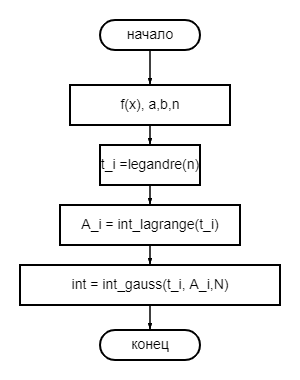
\includegraphics[scale=0.7]{diagram (6).png} 
\end{center}
\caption{Блок-схема метода Гаусса} \label{Рис1}
\end{figure}

\newpage
\section{Численный анализ решения задачи}


\subsection{Исследование зависимости погрешности от степени полинома} 

\begin{figure}[h!]
\begin{center}
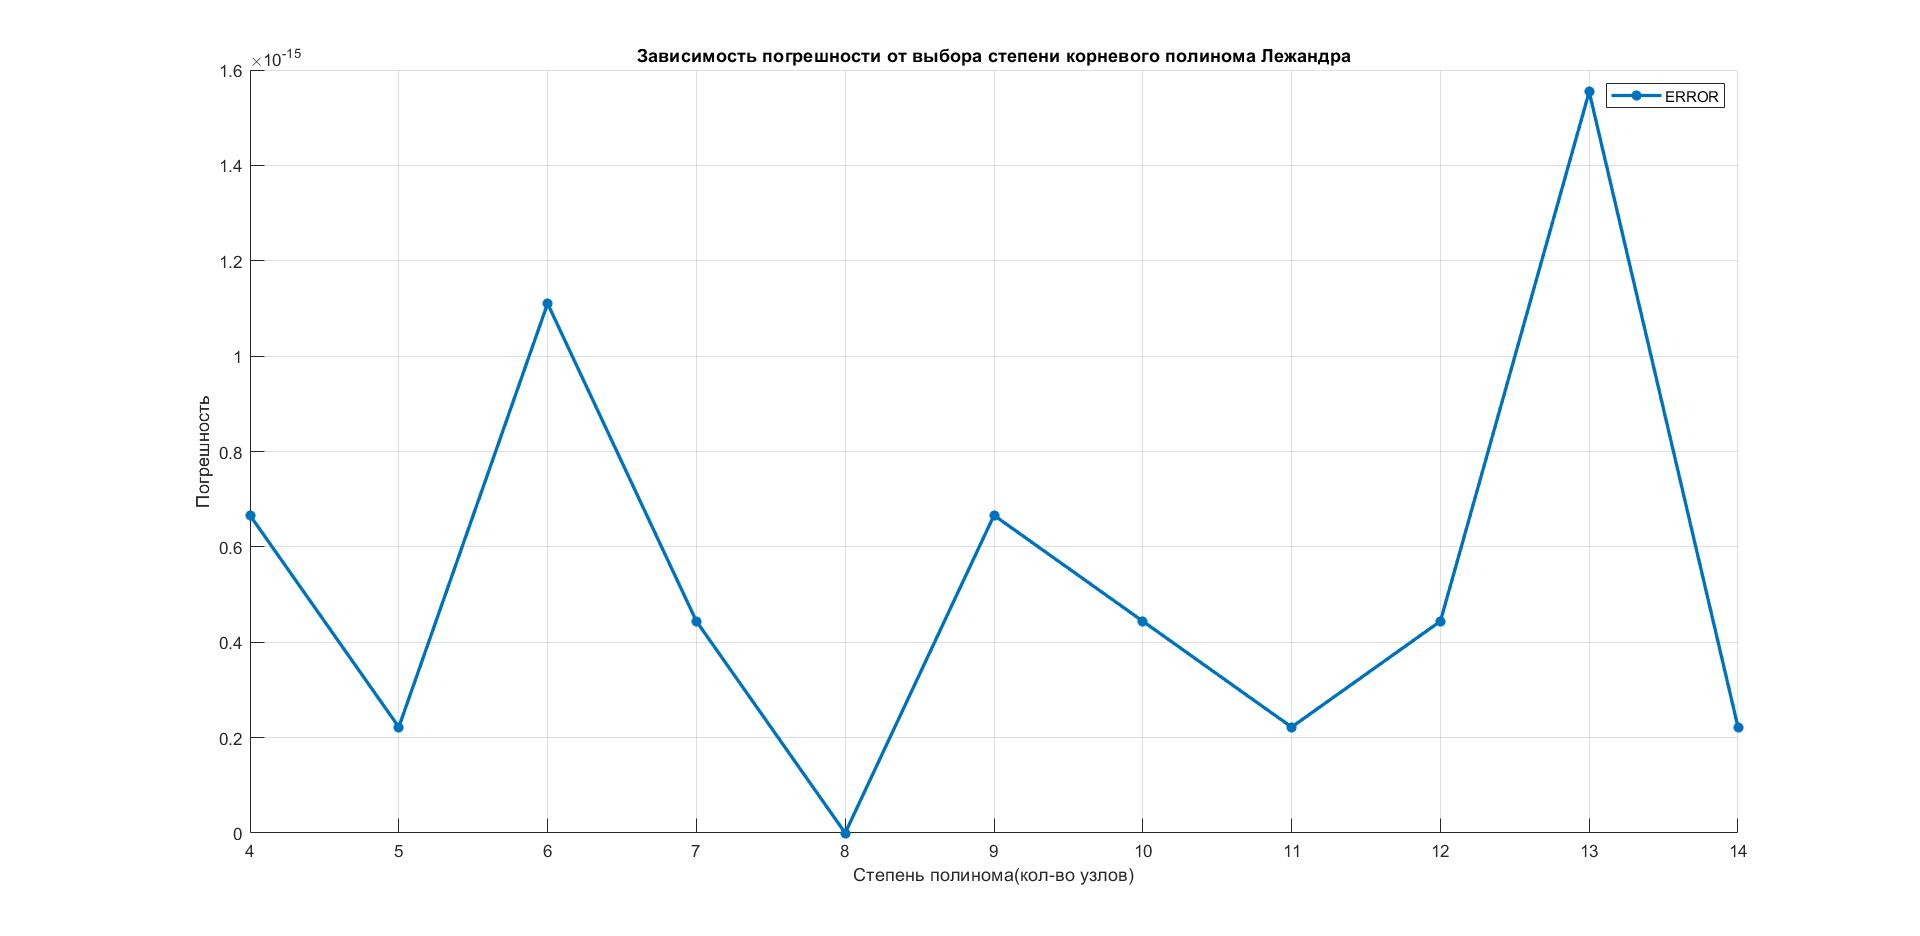
\includegraphics[scale=0.3]{график зависимости погрешности от степени полинома Лежандра.jpg} 
\end{center}
\caption{Зависимость погрешности от степени корневого полинома Лежандра} \label{Рис2}
\end{figure}
На рисунке $\ref{Рис2}$ мы наблюдаем изменение погрешности при изменении степени полинома Лежандра и фиксированном разбиении (отрезок [a,b] не разбит на дополнительные). Определенного закона для погрешности мы не надблюдаем, однако, можно отметить, что погрешность везде очень маленькая, в порядке $10^{-15}$.


\subsection{Сравнение теоретической и фактической точности} 

\begin{figure}[h!]
\begin{center}
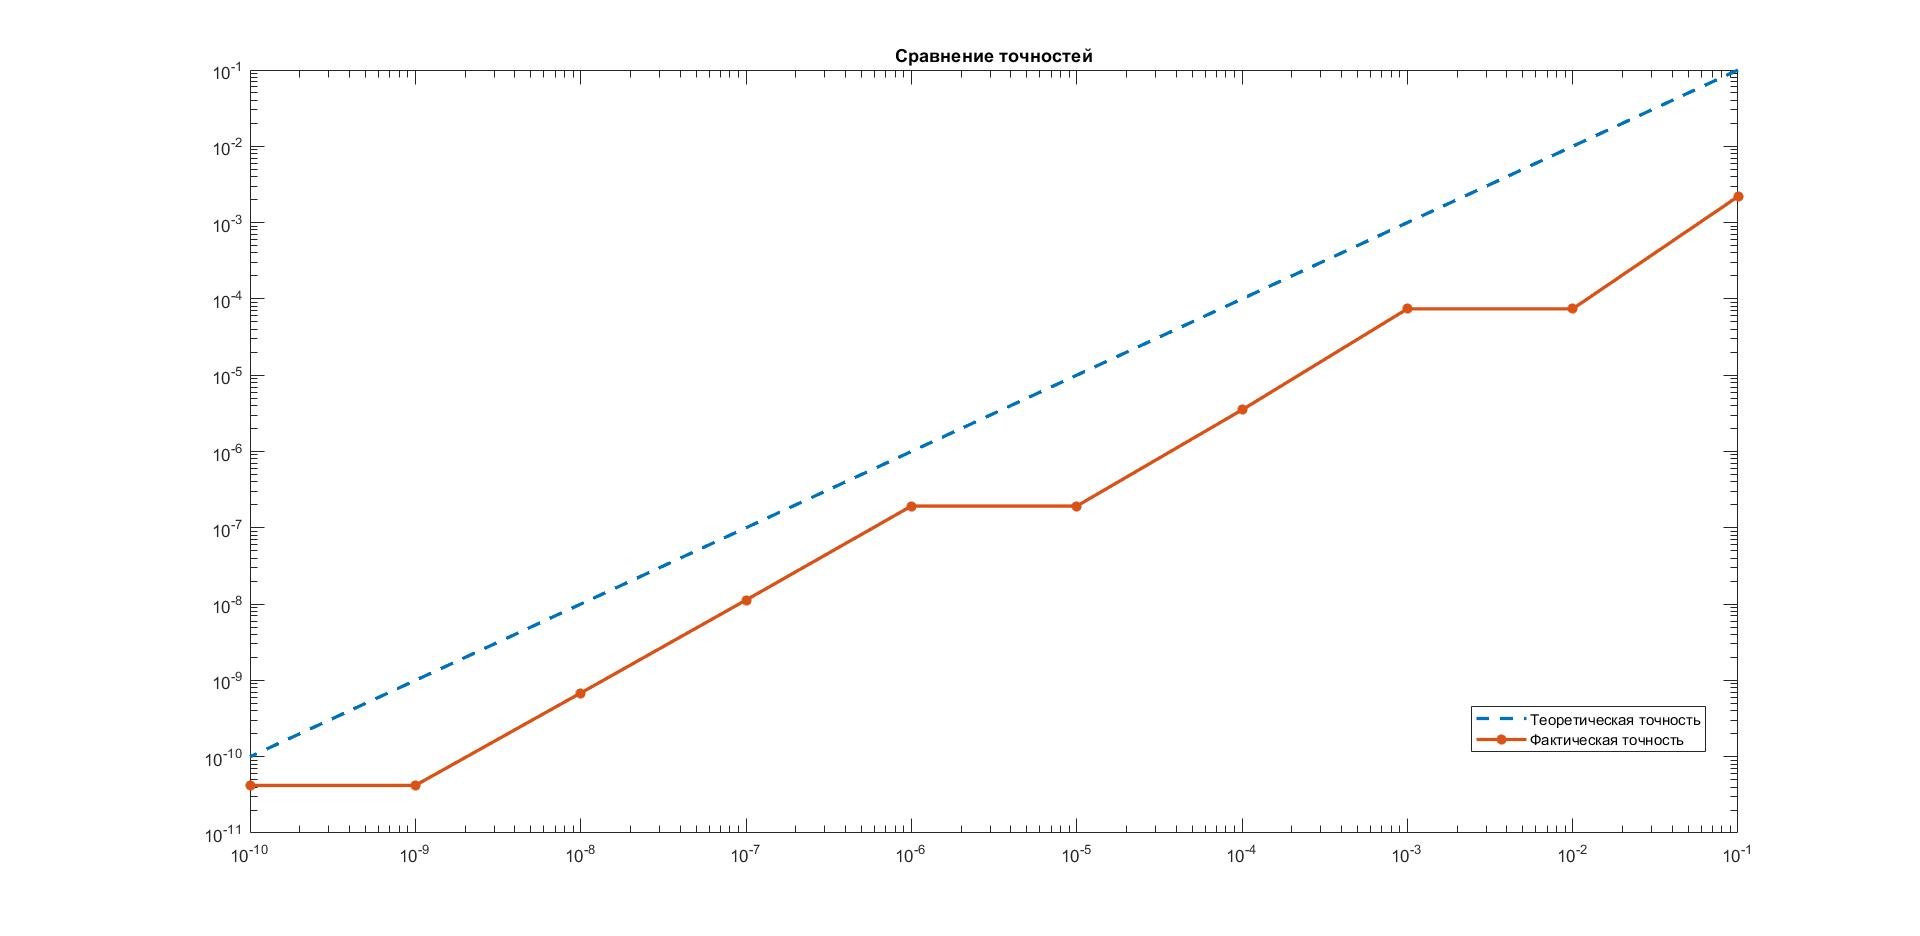
\includegraphics[scale=0.3]{точность.jpg} 
\end{center}
\caption{Сравнение теоретической и фактической точности} \label{Рис3}
\end{figure}
На рисунке $\ref{Рис3}$ можно отметить, что фактическая точность не превышает теоретической, что и ожидалось.\\

\subsection{Исследование влияния разбиений на погрешность}
\begin{figure}[h!]
\begin{center}
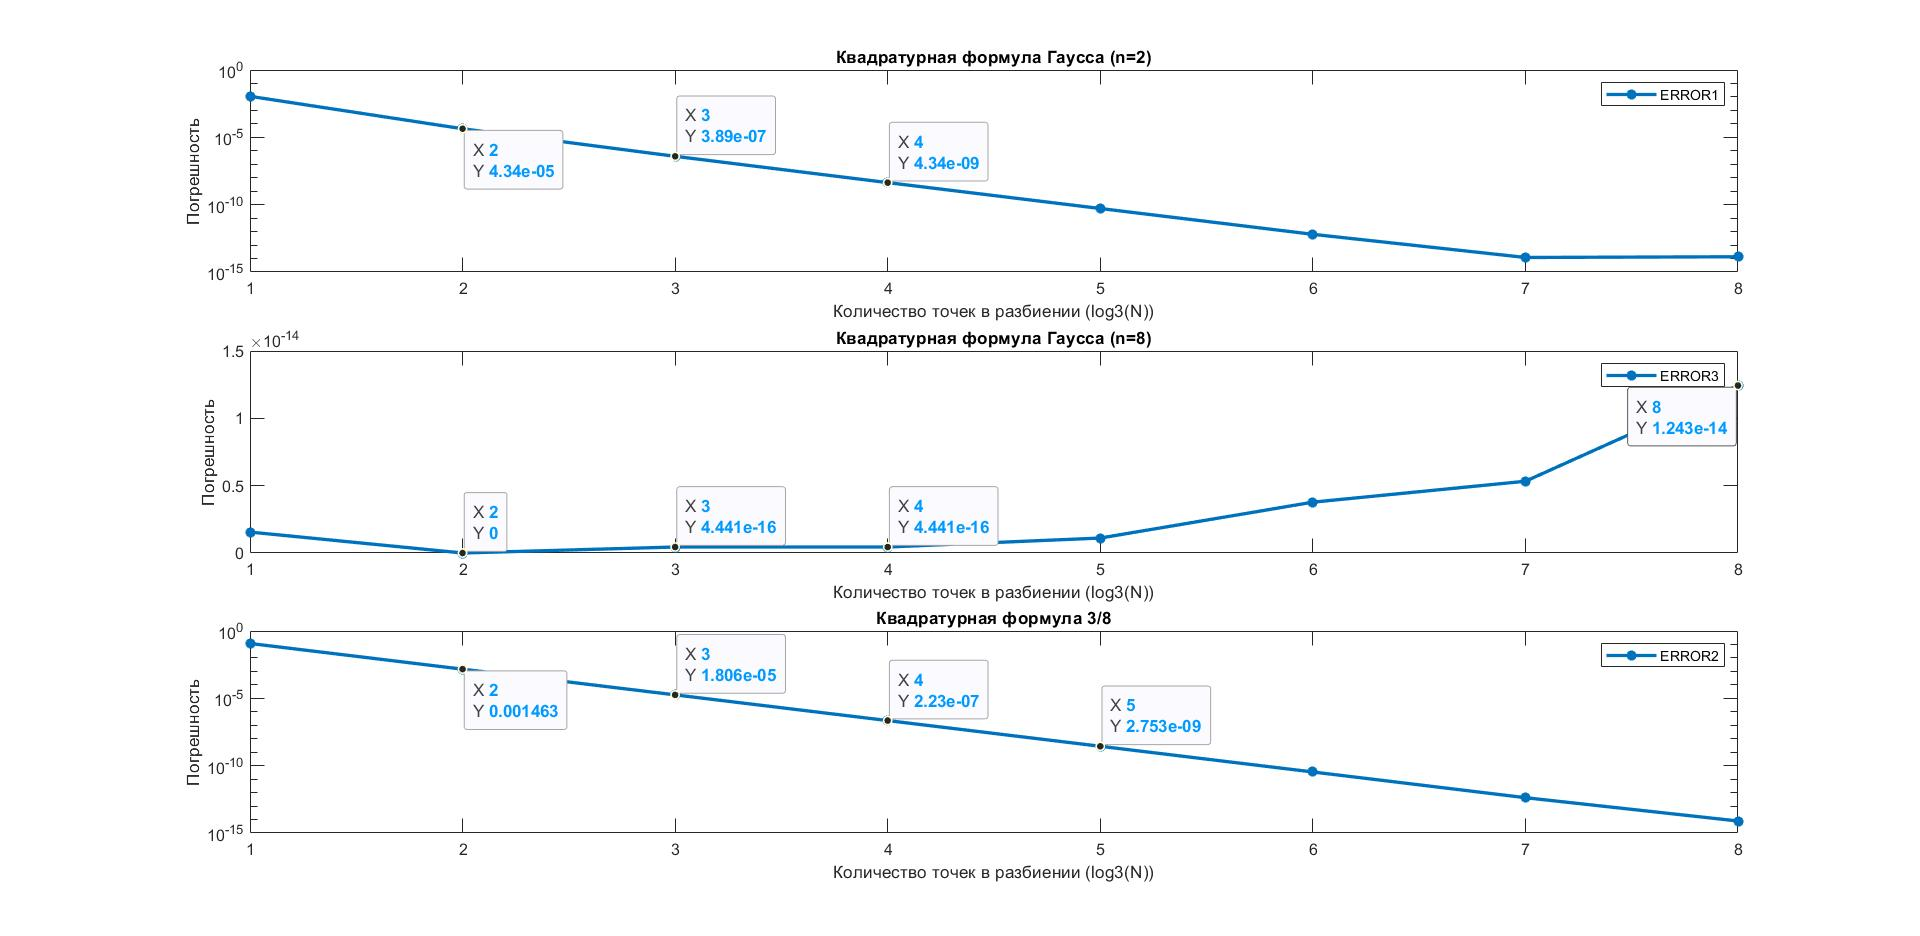
\includegraphics[scale=0.3]{сравнение.jpg} 
\end{center}
\caption{Исследование влияния разбиений на погрешность} \label{Рис4}
\end{figure}
На рисунке $\ref{Рис4}$ мы наблюдаем три графика. По оси абсцисс отмечаем количество точек в разбиении интервала интегрирования, по оси ординат - погрешность. Первый и второй график выполнены при фиксированной степени полинома Лежандра. Первый - степень равна двум, второй - восьми. На первом графике мы видим тенденцию уменьшения погрешности, при увеличении разбиения, погрешность доходит до$10^{-15}$, но изначальное ее значение достаточно большое. Если же мы рассмотри график с фиксированной степенью 8 увидим, что зависимости от степени разбиения не наблюдается, но и изменение погрешности очень мало и колеблется в порядке $10^{-15}$, в самых "лучших" точках погрешность равно нулю, либо порядка $10^{-15}$. 
На третьем графике мы видим уже знакомую зависимость для метода 3/8. Можем заметить, что первый и третий график очень похожи друг на друга.Однако, погрешность на порядок быстрее уменьшается у квадратурных формул Гаусса, что можно видеть из значений точек при равном разбиении.


\newpage
\section{Краткие выводы} 

\begin{itemize}
  \item Квадартурные формулы Гаусса позволяют вычислить интеграл с достаточно высокой точностью, если подобрать "хорошую" степень полинома Лежандра или нужное разбиение.
  \item Все исследования удовлетворили предварительному анализу.
  \item Исследования показали, что для того, чтобы метод дал хорошие результаты, можно брать "большую" степень полинома Лежандра, но для нее не будет известно зависимости погрешноси от разбиения, однако можно получить очень хорошие результаты, подобрав нужное количество точек в разбиении. Неплохой результат дает и "маленькая" степень, где точно известно, что при большом кол-ве разбиений получается маленькая погрешность. 
  \end{itemize}


\end{document} % КОНЕЦ ДОКУМЕНТА !

